%% 한국어 번역본 (검토·공유용). 제출본은 영어 main.tex이다.
%% Overleaf에서 이 파일을 Main document로 지정하고 Compiler를 pdfLaTeX로 둔다. 글꼴 오류가 나면 XeLaTeX로 바꾼다.
\documentclass[twocolumn,10pt]{article}
\usepackage[letterpaper,margin=0.75in,columnsep=0.25in]{geometry}
\usepackage{kotex}
\usepackage[round]{natbib}
\usepackage{graphicx}
\usepackage{amsmath}
\usepackage{amssymb}
\usepackage{booktabs}
\usepackage{xcolor}
\usepackage[small]{caption}
\usepackage{url}

\newcommand{\todo}[1]{\textcolor{red}{[TODO: #1]}}
\newcommand{\pilot}{\textsuperscript{\textcolor{gray}{$\dagger$}}}
\newcommand{\sg}{\operatorname{sg}}
\newcommand{\JS}{\operatorname{JS}}

\title{정책 유사성은 팀 소속이 아니다:\\ 잠재 팀 사이의 선택적 critic 공유 진단}
\author{익명 제출 (한국어 번역본)}
\date{}

\begin{document}
\maketitle

\begin{abstract}
학습하는 agent들이 서로 다른 목표를 가진 잠재 팀에 속해 있을 때, 선택적 공유는 매력적이다. 팀원과 공유하면
학습이 빨라질 수 있지만, 팀원이 아닌 agent와의 공유는 쓸모없거나 해로울 수 있다. 분산 환경에서 자연스러운 방법은
행동이 비슷한 상대를 공유 대상으로 고르는 것이다. 우리는 팀 소속이 숨겨져 있고, 관측이 팀 기준이며, 보상이 개인별인
두 팀 창고 과제에서 이 방법을 연구한다. 대상은 정책 유사도로 gate를 여는 critic distillation 방법(PGCT)으로,
고정된 canonical probe 관측 집합에서 agent들의 행동 분포를 비교한다. 고정 정책 진단에서 probe 기반 정책 유사도는
팀원을 식별하지 못했다(여섯 checkpoint에서 같은 팀 AUROC 0.375--0.500). 반면 agent가 자기 시야 안에서 목격한
작업 사건은 한 episode 안에 모든 팀원을 식별했다. 처음부터 학습한 seed 1개 실험(통계적 결과가 아닌 pilot)에서
gate는 초기에 대부분의 쌍을 허용했지만, 약 2M step 이후에는 거의 다른 팀 agent끼리만 연결했다. 연결된 agent들은
같은 목표가 아니라 비슷한 역할과 숙련도를 가진 쌍이었다. 그럼에도 정답 팀과 critic을 공유한 경우가 이 pilot에서 가장
빠르고 높은 학습곡선을 보였고, 공유 범위가 넓을수록 배송을 배운 agent 수가 늘었다. 같은 seed를 다시 실행하면
공유 방식들은 비트 단위로 재현되지 않았고, 배송 시작 시점이 2백만 step까지 달라졌다. 우리는 행동 유사도가 팀, 역할,
숙련도를 뒤섞는다고 결론짓고, 추론한 팀이 학습을 개선한다고 주장하기 전에 필요한 증거를 정리한다.
\end{abstract}

\section{서론}
많은 다중 agent 시스템에서 환경을 공유하는 agent들이 목표까지 공유하지는 않는다. 서로 다른 고객사의 창고 로봇,
서로 다른 운송사의 차량, 서로 다른 팀의 선수들은 같은 공간에서 움직이고, 서로를 국소적으로 관측하며, 동시에
학습한다. 파라미터, 경험, 가치 추정 같은 학습된 지식을 공유하는 것은 다중 agent 강화학습(MARL)에서 표본 효율을
높이는 잘 알려진 방법이다~\cite{christianos2020seac,christianos2021seps}. 하지만 이는 공유하는 agent들이 서로
호환된다는 전제를 깔고 있다. 팀 소속이 숨겨져 있다면, agent는 먼저 \emph{누구와} 공유할지 정해야 한다.

분산 환경에서 끌리는 답은 \emph{행동}이 비슷한 agent와 공유하는 것이다. 우리가 분석하는 방법인 정책 gate 기반 critic
전이(PGCT)가 이 아이디어를 따른다. agent들은 고정된 probe 관측 집합에서 행동 분포를 비교하고, 정책이 충분히 가까운
이웃의 critic을 distillation한다. 이 아이디어는 세 가정에 기대고 있다. (i) 팀원은 다른 팀보다 행동이 더 비슷하다.
(ii) probe 집합이 그 차이를 드러낸다. (iii) 팀원의 가치 함수가 더 호환되므로 그들의 critic이 유용한 목표가 된다.
각 고리는 끊어질 수 있다. 팀원끼리 역할이 다를 수 있고, 다른 팀이 대칭적인 하위 문제를 같은 방식으로 풀 수 있으며,
개인 보상에서는 팀원끼리 같은 요청을 두고 경쟁한다.

이 논문은 통제된 환경에서 이 가정의 사슬을 진단한다. 세 질문을 분리한다.
\begin{itemize}
  \item \textbf{RQ1(식별 가능성).} agent가 가진 정보로 팀원을 식별할 수 있는가? probe 기반 정책 유사도가 그 정보를 담고 있는가?
  \item \textbf{RQ2(올바른 상대의 가치).} 처음부터 학습할 때, 정답 팀과 critic을 공유하는 것이 공유하지 않는 경우나 모두와
    공유하는 경우보다 도움이 되는가?
  \item \textbf{RQ3(gate의 실제 동작).} 학습 중 유사도 gate는 실제로 어떤 상대를 고르며, 그 이유는 무엇인가?
\end{itemize}

기여는 다음과 같다. (1) 팀 식별 가능성, 정답 팀 공유의 가치, 추론된 gate의 동작을 서로 분리하는 문제 정식화와 평가
절차. 실제 donor 할당은 매 update 기록한다. (2) 팀 대칭적 창고 과제에서 probe 기반 정책 유사도는 팀을 식별하지 못하고,
국소적으로 목격한 작업 사건은 식별한다는 증거. (3) 처음부터 학습한 pilot. 유사도 gate가 비슷한 역할의 다른 팀 agent
연결로 옮겨 가는 반면, 정답 팀 공유는 가장 좋은 학습곡선을 보이고 공유 범위가 넓을수록 더 많은 agent가 학습한다.
(4) 같은 seed와 초기 가중치에서도 공유 방식들이 비트 단위로 재현되지 않음을 보이는 재현성 분석. 어떤 결과가 seed 1개
pilot인지, 무엇이 아직 빠졌는지(다중 seed, 목표 분리 환경, 온라인 팀 추론 방법)를 명시한다.

\section{관련 연구}
\textbf{MARL에서의 공유.} 협력 MARL에서 파라미터 공유는 표준적이다. SePS는 transition의 학습된 인코딩으로 agent를
군집화하고 군집 안에서 파라미터를 공유한다~\cite{christianos2021seps}. 이질성을 고려하는 방법은 어떤 agent끼리 공유할지
동적으로 정한다~\cite{hu2025heterogeneity}. SEAC는 importance weighting으로 서로의 경험에서 배우게 한다
\cite{christianos2020seac}. 이 연구들은 주로 모든 agent가 공통 목표를 최적화하는 협력 상황을 다룬다. 우리는 목표 집단
소속이 숨겨져 있고, critic 예측만 공유하며, actor는 독립적으로 유지되는 경우를 다룬다.

\textbf{분산 critic.} 네트워크 actor-critic 방법은 통신 그래프 위에서 critic 파라미터의 합의에 도달하며, 선형 근사에서
수렴이 보장된다~\cite{zhang2018networked}. 우리 설정에서는 통신 그래프(물리적 근접)와 팀 구조가 다르고, 보상이
개인별이며, critic은 recurrent 신경망이고 distillation 손실로 probe 입력에서만 맞춰진다~\cite{rusu2016policy}.

\textbf{역할과 독립 학습.} RODE 같은 역할 기반 방법은 행동의 효과로 역할을 발견한다~\cite{wang2021rode}. 역할과 팀은
서로 다른 잠재 변수다. 팀원끼리 역할이 다를 수 있고 다른 팀끼리 역할이 같을 수 있는데, 이것이 바로 우리가 관찰한
혼동이다. 우리의 학습자는 독립 recurrent PPO agent다~\cite{schulman2017ppo,dewitt2020ippo}. MAPPO
\cite{yu2022mappo}는 중앙 critic을 쓰며, 이후 단계의 자연스러운 baseline이다. 평가 절차는 \cite{agarwal2021precipice}의
권고를 따른다.

\section{문제 설정}
agent $i\in\{1,\dots,N\}$, 국소 관측 이력 $h_i^t$, 행동 $a_i^t$, 개인 보상 $r_i^t$를 가진 부분관측 확률 게임을 고려한다.
각 agent는 자신의 목표(어떤 요청을 처리하고 어디로 배송하는지)를 결정하는 잠재 팀 $z_i\in\{1,\dots,K\}$에 속한다.
agent는 팀 기준 관측 채널을 통해 자기 목표를 알지만, 다른 agent의 $z_j$는 관측하지 못한다. 통신 범위 안의 agent들은
시간에 따라 바뀌는 이웃 $\mathcal{N}_i(t)$를 이루며, 미리 합의한 공통 probe 집합에 대한 모델 출력을 교환할 수 있다.
원시 관측이나 팀 라벨은 교환하지 않는다.

\textbf{환경.} 다중 로봇 창고(RWARE)~\cite{papoudakis2021benchmarking}의 두 팀 변형을 $11\times10$ 맵(\emph{E1})에서
agent 4명으로 사용한다(agent 1, 3은 빨강 팀, 2, 4는 파랑 팀). 각 팀은 항상 요청 선반 2개와 자기 배송 목표를 가진다.
두 목표는 맵 아래 가운데에 붙어 있다. 각 팀 선반의 절반은 상대 팀 구역에 놓인다. 관측은 자기 중심
$11\times11$ semantic grid와 ego feature이며, ``요청 선반''과 ``해당 목표'' 같은 채널은 관측자의 팀 기준으로 정의된다.
보상은 개인별이다. agent는 자기 팀 요청 선반을 직접 배송·반납할 때와 작은 shaping 항에서만 보상을 받는다. 팀 기준
관측과 인접한 목표 때문에 두 팀은 같은 결정 문제를 푼다. 따라서 E1은 팀 정체성이 가치 예측에 거의 중요하지 않은
\emph{팀 대칭} 조건이다. 또 목표를 맵 아래 양쪽 모서리로 옮긴 \emph{E1-F}를 정의한다. E1-F에서는 목표가 시야에 없을 때
두 팀의 올바른 행동이 갈라진다.

\section{비교 방법}
모든 방법은 무작위 초기화에서 학습하는 독립 recurrent PPO actor와 critic(GRU 128 unit)을 쓴다. 같은 seed에서는 모든
방법이 비트 단위로 같은 가중치에서 시작한다. 차이는 보조 critic distillation 항뿐이다. $\mathcal{Q}=\{q_m\}_{m=1}^{M}$을
고정 probe 관측 집합이라 하자($M=48$, 환경 배치에서 결정적으로 생성, 시퀀스 길이 1, hidden state 0으로 시작).
donor 가중치 $\alpha_{ij}$를 가진 receiver $i$의 손실은
\begin{equation}
  \mathcal{L}_i = \mathcal{L}^{\mathrm{PPO}}_i + \lambda_{\mathrm{peer}} \sum_{j\in\mathcal{N}_i(t)} \alpha_{ij}\,
  \frac{1}{M}\sum_{m=1}^{M}\big(V_i(q_m) - \sg[V_j(q_m)]\big)^2
\end{equation}
이다. $\lambda_{\mathrm{peer}}=0.01$이고 $\sg$는 stop-gradient다. 방법들은 gate $g_{ij}\in\{0,1\}$만 다르며,
$\alpha_{ij}=g_{ij}/\sum_k g_{ik}$는 현재 이웃에 대해 정규화한다.
\begin{itemize}
  \item \textbf{IPPO}: distillation 없음($g_{ij}=0$).
  \item \textbf{Oracle-team}: $g_{ij}=\mathbf{1}[z_i=z_j]$(특권 정보를 쓰는 참조 기준이며 상한이 아니다).
  \item \textbf{All-peer}: 모든 이웃에 대해 $g_{ij}=1$.
  \item \textbf{PGCT}: 5 update마다 이웃끼리 probe 집합에서 정책을 비교한다.
  \begin{equation}
    D_{ij} = \frac{1}{M}\sum_{m=1}^{M} \JS\big(\pi_i(\cdot\mid q_m),\, \pi_j(\cdot\mid q_m)\big)
  \end{equation}
  지수이동평균 $\bar D_{ij}\leftarrow(1-\beta)\bar D_{ij}+\beta D_{ij}$($\beta=0.35$)를 유지하고, 100 update warm-up과
  최소 8회 측정 뒤 $g_{ij}=\mathbf{1}[\bar D_{ij}<\tau]$($\tau=0.12$)로 gate를 연다.
\end{itemize}
실제 할당 $\alpha$를 매 update 기록한다. 아래의 ``전이''는 gate 후보가 아니라 실제로 일어난 distillation을 뜻한다.

\section{RQ1: 팀 소속은 식별 가능한가?}
\textbf{절차.} 이전 커리큘럼·연장 학습에서 얻은 checkpoint 6개(E1과 더 큰 맵 E2, training seed 1개)를 고정하고, 각 정책을
500 step episode 20회 실행했다. agent 쌍마다 다음을 계산했다. canonical 집합에서의 probe-JS, 두 agent 자신의 관측 이력에서
두 정책 사이의 이력-JS, 방문 칸 분포 사이의 JS, 그리고 \emph{국소 작업 증거}다. 국소 작업 증거는 다른 agent의 pickup과
배송 가운데 관측자 자신의 $11\times11$ 시야에 들어온 것을, 관측자의 팀 기준 채널(``이 선반은 우리 팀 요청인가?'',
``이 목표는 내 것인가?'')로 분류한 것이다. 2{,}146개 사건에서 세어진 모든 사건이 관측자의 실제 관측에 보이고 올바르게
분류됨을 확인했다. 팀 라벨은 채점에만 쓴다.

\begin{table}[t]
\centering
\small
\resizebox{\columnwidth}{!}{%
\begin{tabular}{lcccc}
\toprule
모델 & Probe-JS & 이력-JS & 방문 분포 & 국소 증거 \\
\midrule
Stage03 (E1) & .500 & .282 & .379 & 1.000 \\
E1 IPPO & .375 & .267 & .408 & 1.000 \\
E1 PGCT & .375 & .267 & .333 & 1.000 \\
E2 IPPO & .375 & .810 & .867 & 1.000 \\
E2 PGCT & .500 & .853 & .821 & 1.000 \\
Stage04 PGCT & .500 & .291 & .365 & 1.000 \\
\bottomrule
\end{tabular}}
\caption{쌍별 점수의 같은 팀 AUROC(1 = 팀원이 항상 더 높음, 0.5 = 우연). training seed 1개의 고정 checkpoint, 각 20$\times$500 step.}
\label{tab:identifiability}
\end{table}

\textbf{결과.} 표~\ref{tab:identifiability}에서 국소 작업 증거는 모든 checkpoint에서 팀원을 완벽하게 구분했고, 첫 episode
안에 모든 팀원을 식별했다. probe-JS는 우연 수준 이하(0.375--0.500)이며, E1 checkpoint의 이력-JS는 우연보다
\emph{낮다}(0.27--0.29). 즉 팀원끼리 오히려 덜 비슷하게 행동한다. 더 큰 맵(E2)에서는 이력과 방문 분포가 팀 정보를
담지만(0.81--0.87), probe 집합은 그렇지 않다.

canonical 집합의 두 성질이 이를 일부 설명한다. 48개 입력 중 서로 다른 것은 26개뿐이고, 중복을 제거하면 쌍의 순위가
바뀐다. 더 근본적으로, 팀 기준 채널에서는 목표가 보이는 probe가 \emph{어느} actor에게나 ``네 목표는 여기''라고 알려
주므로 두 팀이 똑같이 반응한다. 그리고 집합에는 요청 선반을 들고 있으면서 목표가 보이지 않는 probe가 하나도 없다.
팀이 학습한 목표 위치가 영향을 줄 수 있는 유일한 상황인데 말이다. 그래서 이런 ``적재 중, 목표 안 보임'' probe 48개로
검증된 집합을 새로 만들었다. 고정된 E1 모델 4개와 probe 부분집합 5개(새 집합 포함)의 20개 조합 모두에서 팀원 사이의
평균 probe-JS가 팀원이 아닌 쌍보다 컸다(부록~\ref{app:frozen}). E1에서는 두 팀의 목표가 너무 비슷해서 어떤 probe
설계로도 드러나지 않는다.

\textbf{가치 호환성.} 팀원의 critic이 더 좋은 목표라는 전제도 E1에서 성립하지 않았다. receiver 자신의 초기 return에서
계산한 blend gain $\mathrm{MSE}(V_i,G_i)-\mathrm{MSE}(\tfrac12(V_i+V_j),G_i)$의 같은 팀 AUROC는 E1 checkpoint에서
0.25--0.33, E2에서 약 0.5였다. 개인 보상과 대칭 과제에서는 같은 팀이라는 사실이 더 호환되는 가치 예측을 뜻하지 않는다.

\section{RQ2와 RQ3: 처음부터 학습}
\textbf{절차.} IPPO, PGCT, Oracle-team, All-peer를 E1에서 무작위 초기화로 training seed 1개(같은 초기 가중치)로 학습했다.
51{,}200 step마다 deterministic masked 정책으로, 고정 reset seed의 500 step episode 20회를 평가했다. 15M step으로
계획했으나 약 6.5M에서 멈췄고, 모든 통계는 공통 구간 6.4M step을 쓴다. \emph{이 결과는 seed 1개의 pilot이다}(\pilot{} 표시).
하이퍼파라미터는 부록~\ref{app:hyper}에 있다.

\begin{figure}[t]
\centering
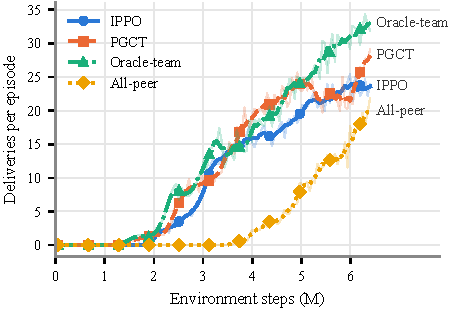
\includegraphics[width=\columnwidth]{figures/fig1_learning_curves.pdf}
\caption{E1에서 무작위 초기화로 학습하는 동안의 평가 배송 수/episode(training seed 1개). 가는 선: 51{,}200 step마다의
원 평가값, 굵은 선: 중심 5점 이동평균.}
\label{fig:curves}
\end{figure}

\begin{table}[t]
\centering
\small
\resizebox{\columnwidth}{!}{\begin{tabular}{lcccccc}
\toprule
Method & \multicolumn{3}{c}{Onset (M steps)} & Mean deliv. & Final deliv. & Agents \\
\cmidrule(lr){2-4}
 & $\geq$1 & $\geq$10 & $\geq$20 & 0--6.4M & (last 5 evals) & learned \\
\midrule
IPPO & 2.05 & 3.17 & 5.07 & 10.4 & 23.2 $\pm$ 1.1 & 2/4 \\
PGCT & 1.79 & 3.28 & 4.15 & 11.7 & 27.3 $\pm$ 1.4 & 3/4 \\
Oracle-team & 1.64 & 2.97 & 4.66 & 13.2 & 32.2 $\pm$ 1.7 & 3/4 \\
All-peer & 3.99 & 5.32 & -- & 3.7 & 19.4 $\pm$ 1.6 & 4/4 \\
\bottomrule
\end{tabular}
}
\caption{E1 pilot 결과\pilot{}(seed 1개, 공통 구간 6.4M). Onset: episode당 배송의 3점 이동평균이 해당 수준에 처음 도달한
step. Final: 마지막 평가 5회의 평균 $\pm$ 표준편차. Agents learned: 마지막 평가 5회에서 episode당 1개 이상 배송한 agent 수.}
\label{tab:performance}
\end{table}

\textbf{학습곡선.} Oracle-team 공유가 가장 이른 시작과 가장 높은 곡선을 보였다(그림~\ref{fig:curves}, 표~\ref{tab:performance}).
episode당 배송 1개에 도달한 시점은 1.64M step으로 IPPO의 2.05M보다 빨랐고, 학습 중 평균 배송은 13.2 대 10.4, 마지막은
32.2 대 23.2였다. PGCT는 그 사이였다. All-peer 공유는 학습을 약 2백만 step 늦췄지만 마지막에 가장 빠르게 오르고 있었다.\pilot

\begin{figure*}[t]
\centering
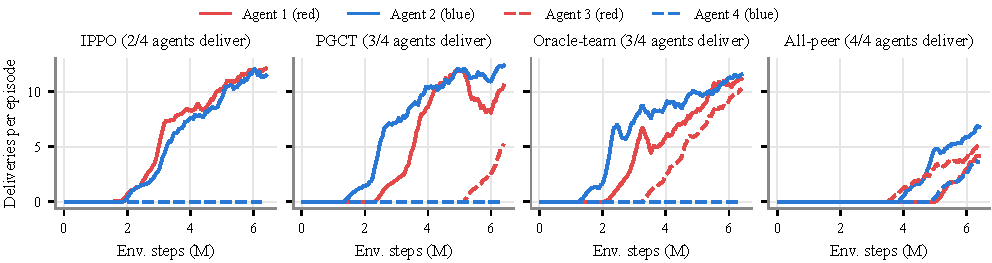
\includegraphics[width=\textwidth]{figures/fig2_per_agent_deliveries.pdf}
\caption{agent별 배송 수/episode(5점 이동평균). 빨강: 빨강 팀(agent 1, 3), 파랑: 파랑 팀(agent 2, 4). 실선: agent 1--2,
점선: agent 3--4. 패널 제목은 배송하는 agent 수다.}
\label{fig:agents}
\end{figure*}

\textbf{공유가 몇 명이 배우는지를 정한다.} 처리량 차이의 대부분은 배송을 아예 배운 agent 수로 설명된다(그림~\ref{fig:agents}).
IPPO는 2명(팀당 1명), PGCT와 Oracle-team은 3명, All-peer는 4명이다. 배운 agent 한 명은 episode당 약 10--12개를 배송했다.
배우지 못한 agent는 계속 움직였지만 평가에서 요청 선반을 한 번도 집지 않았다. 그럴듯한 메커니즘은 다음과 같다. 개인 보상이고
팀당 요청이 2개뿐이라, 먼저 배운 팀원이 요청 대부분을 처리하고 다른 팀원은 배울 만큼의 보상을 받지 못한다. 유능한 동료의
critic을 distillation하면 자기 보상 없이도 학습 신호가 생긴다. Oracle-team에서 agent 1의 뒤처진 팀원은 3.6M step에 배송을
시작했지만, IPPO에서 해당 agent는 끝내 배우지 못했다. 그러나 공유만으로 충분하지는 않다. Oracle-team의 agent 4는
agent 2로부터 꾸준히 distillation을 받았는데도 배우지 못했다.\pilot{} 이 메커니즘은 가설이다. 검증하려면 seed 반복과 개입
실험(예: 뒤처진 agent의 distillation 차단)이 필요하다.

\begin{figure*}[t]
\centering
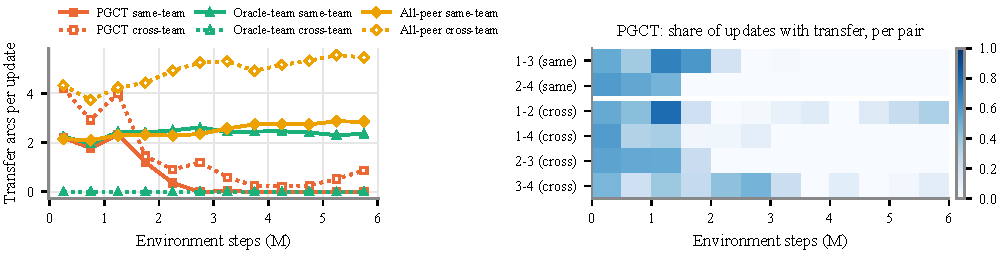
\includegraphics[width=\textwidth]{figures/fig3_critic_transfer.pdf}
\caption{실제 critic 전이(기록된 donor 할당, warm-up 이후). 왼쪽: update당 방향성 전이 arc 수, 같은 팀(실선)과 다른 팀(점선),
0.5M step 구간 평균. 오른쪽: PGCT에서 각 쌍이 critic 정보를 주고받은 update 비율.}
\label{fig:transfer}
\end{figure*}

\begin{table}[t]
\centering
\small
\resizebox{\columnwidth}{!}{\begin{tabular}{llccc}
\toprule
Method & Window & Updates w/ transfer & Same-team arcs/upd. & Cross-team arcs/upd. \\
\midrule
PGCT & 0--2.0M & 91\% & 1.86 & 3.09 \\
 & 2--4.0M & 37\% & 0.10 & 0.73 \\
 & 4--6.4M & 29\% & 0.03 & 0.63 \\
\addlinespace
Oracle-team & 0--2.0M & 82\% & 2.26 & 0.00 \\
 & 2--4.0M & 86\% & 2.50 & 0.00 \\
 & 4--6.4M & 85\% & 2.39 & 0.00 \\
\addlinespace
All-peer & 0--2.0M & 99\% & 2.22 & 4.18 \\
 & 2--4.0M & 100\% & 2.49 & 5.10 \\
 & 4--6.4M & 100\% & 2.79 & 5.37 \\
\bottomrule
\end{tabular}
}
\caption{학습 구간별 실제 전이(seed 1개\pilot). arc는 receiver--donor 방향 연결이다.}
\label{tab:transfer}
\end{table}

\textbf{gate가 고르는 상대(RQ3).} 처음 2M step 동안 PGCT gate는 update의 91\%에서 전이를 허용했다. 모든 정책이 아직
비슷하기 때문에 다른 팀 전이(update당 3.09 arc)가 같은 팀(1.86)보다 많았다(그림~\ref{fig:transfer}, 표~\ref{tab:transfer}).
2M step부터는 같은 팀 전이가 거의 사라졌고(2--4M에 0.10, 4--6.4M에 0.03 arc/update), 남은 연결은 다른 팀끼리였다.
처음에는 agent 3과 4, 나중에는 가장 많이 배송한 두 agent인 1과 2가 연결됐다. 2.5M step 이후 거의 모든 checkpoint에서,
네 방법 모두 팀원 사이의 probe-JS가 팀원이 아닌 쌍보다 컸다(그림~\ref{fig:jsgap}). 정답 팀 안에서 critic을 공유해도
팀원의 actor가 더 비슷해지지 않았다.

\begin{figure}[t]
\centering
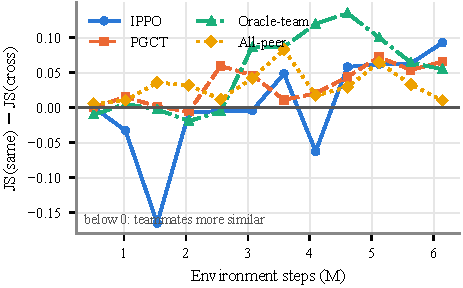
\includegraphics[width=\columnwidth]{figures/fig4_probe_js_gap.pdf}
\caption{48개 canonical probe에서 팀원 사이 probe-JS에서 팀원이 아닌 쌍의 probe-JS를 뺀 값(checkpoint에서 계산). 0보다
크면 팀원의 정책이 팀원이 아닌 쌍보다 덜 비슷하다.}
\label{fig:jsgap}
\end{figure}

\textbf{팀이 아니라 역할.} 이전 커리큘럼 모델(선반의 50\%를 상대 팀 구역에 둔 조건)을 고정해 분석하면, gate가 포착하는
구조가 보인다(부록~\ref{app:roles}). agent 1과 2는 거의 자기 팀 구역에서만 일했다(step의 99.6\%, 99.5\%). 반면 agent
3과 4는 자기 팀 요청 선반 대부분을 상대 구역에서 가져왔고, 시간의 약 76\%를 운반에 썼다. 두 ``원거리 운반'' agent는
서로 다른 팀이지만 비슷하게 행동하며, gate가 가장 많이 연결한 쌍이었다(1{,}170 update). 같은 커리큘럼에서 같은 팀
gate 거리는 각 팀 선반이 자기 구역에만 있을 때 0.086과 0.100이었고, 선반을 12.5\%만 섞어도 0.26과 0.32로 올랐다.
따라서 행동 유사도는 역할과 숙련도를 따르며, E1에서 이것들은 팀 소속과 일치하지 않는다.

\textbf{재현성.} 같은 seed와 같은 초기 가중치로 다시 실행하면 IPPO는 정확히 재현됐다(2.46M step까지 평가 곡선 동일).
하지만 세 공유 방식은 1.38--1.59M step 이후 이전 실행과 갈라졌다(부록~\ref{app:repro}). distillation 경로의 비결정적
GPU 연산 때문으로 추정하지만 아직 확인하지 않았다. 차이는 컸다. All-peer의 배송 시작 시점이 1.89M에서 3.99M step으로
바뀌었다. 따라서 공유 방식 사이의 비교에는 독립 seed 여러 개가 필요하다.

\section{논의}
\textbf{증거가 뒷받침하는 것.} (i) 팀 대칭 과제에서 probe 기반 정책 유사도는 팀을 식별하지 못하고 역할과 숙련도에 지배된다.
이는 고정 checkpoint, probe 설계, 처음부터 학습한 실행 모두에서 성립했다. (ii) 팀을 실제로 식별하는 정보, 즉 국소적으로
목격한 작업 사건은 명시한 관측 가정 아래에서 agent가 사용할 수 있다. (iii) seed 1개에서 정답 팀과의 critic 공유가 가장 좋은
학습곡선을 보였고, 더 넓은 공유는 더 많은 agent가 배우게 했다. 둘 다 반복 검증이 필요하다.

\textbf{증거가 뒷받침하지 않는 것.} PGCT나 다른 추론 팀 방법이 학습을 개선한다거나, 정답 팀 공유가 안정적으로 도움이 된다거나,
관찰된 메커니즘(뒤처진 agent 구제)이 인과적이라고 주장하지 않는다. E1에서 probe-JS가 실패한 것은 과제 대칭성에서 예상되는
결과이며, 팀 목표가 다를 때는 달라질 수 있다.

\textbf{가정.} 국소 작업 증거를 쓰려면 관측자가 관측한 사건을 특정 이웃에게 귀속할 수 있어야 하고(관측 grid에는 agent 식별자가
없다), 자기 목표를 알아야 한다. agent들이 팀 식별자를 그냥 주고받을 수 있다면 팀 추론은 필요 없다. 이 설정은 목표가 비공개이거나,
조직 간에 라벨이 공유되지 않거나, 공통 어휘 없이 집단이 생겨날 때 의미가 있다. 분산 팀 발견을 주장하려면 이 가정을 명시해야 한다.

\textbf{다음 단계.} \todo{실행이 끝나면 채운다.} (1) E1 비교의 seed 2--3(이상). 배운 agent 수를 명시적 지표로 쓴다.
(2) 팀 목표를 양쪽 모서리에 둔 E1-F. 팀 행동이 갈라지는가, ``적재 중, 목표 안 보임'' probe 집합이 팀을 구분하는가,
팀의 가치 함수가 다를 때 Oracle-team 공유가 All-peer보다 이득을 보는가? (3) probe 유사도 대신 국소 작업 증거로 움직이는 온라인
gate를 Oracle-team, All-peer, IPPO와 비교. (4) 안정적인 효과가 있는 조건을 확정한 뒤 MAPPO와 SePS 방식 baseline.

\section{결론}
행동 유사도는 누구와 공유할지 정하는 매력적인 분산 대리 지표다. 하지만 우리 창고 연구에서 이것은 팀 소속이 아니라 역할과
숙련도를 측정했다. 유사도 gate 기반 critic 공유 방법은 점차 다른 팀 agent끼리 연결했고, 국소적으로 목격한 작업 결과는 팀을 즉시
식별했다. 올바른 상대와의 공유는 pilot에서 이로워 보였고, 주로 뒤처진 agent의 학습을 도왔다. 추론한 팀이 학습을 개선한다는
것을 보이려면 식별 가능성, 정답 팀 공유의 가치, 추론된 gate의 동작을 분리해야 한다. 또 공유 방식은 작은 수치 차이를 증폭하므로
여러 seed가 필요하다.

\bibliographystyle{plainnat}
\bibliography{references}

\clearpage
\appendix
\onecolumn

\section{하이퍼파라미터}
\label{app:hyper}
\begin{table}[h]
\centering
\small
\begin{tabular}{ll}
\toprule
Setting & Value \\
\midrule
Map / agents / teams & 11$\times$10 E1 / 4 / 2 \\
Reward & individual \\
Home-zone shelf ratio & 0.5 \\
Requests per team & 2 \\
Sensor / communication range & 5 / 5 \\
Learning rate & 0.0002 \\
Entropy coef. & 0.05 \\
$\gamma$ / GAE $\lambda$ & 0.99 / 0.95 \\
Rollout / BPTT length & 1024 / 64 \\
PPO epochs / minibatches / clip & 4 / 8 / 0.2 \\
Hidden (MLP / GRU) & 128 / 128 \\
Peer-loss coef. $\lambda_{peer}$ & 0.01 \\
Gate: JS threshold / EMA $\beta$ / warm-up & 0.12 / 0.35 / 100 upd. \\
Canonical probes & 48 (fixed, zero hidden, length 1) \\
Evaluation & every 50 updates, 20$\times$500 steps, deterministic \\
\bottomrule
\end{tabular}

\caption{처음부터 학습한 E1 비교의 설정(distillation gate를 제외하고 모든 방법이 동일).}
\end{table}

\section{고정 E1 모델에서의 probe 집합}
\label{app:frozen}
\begin{figure}[h]
\centering
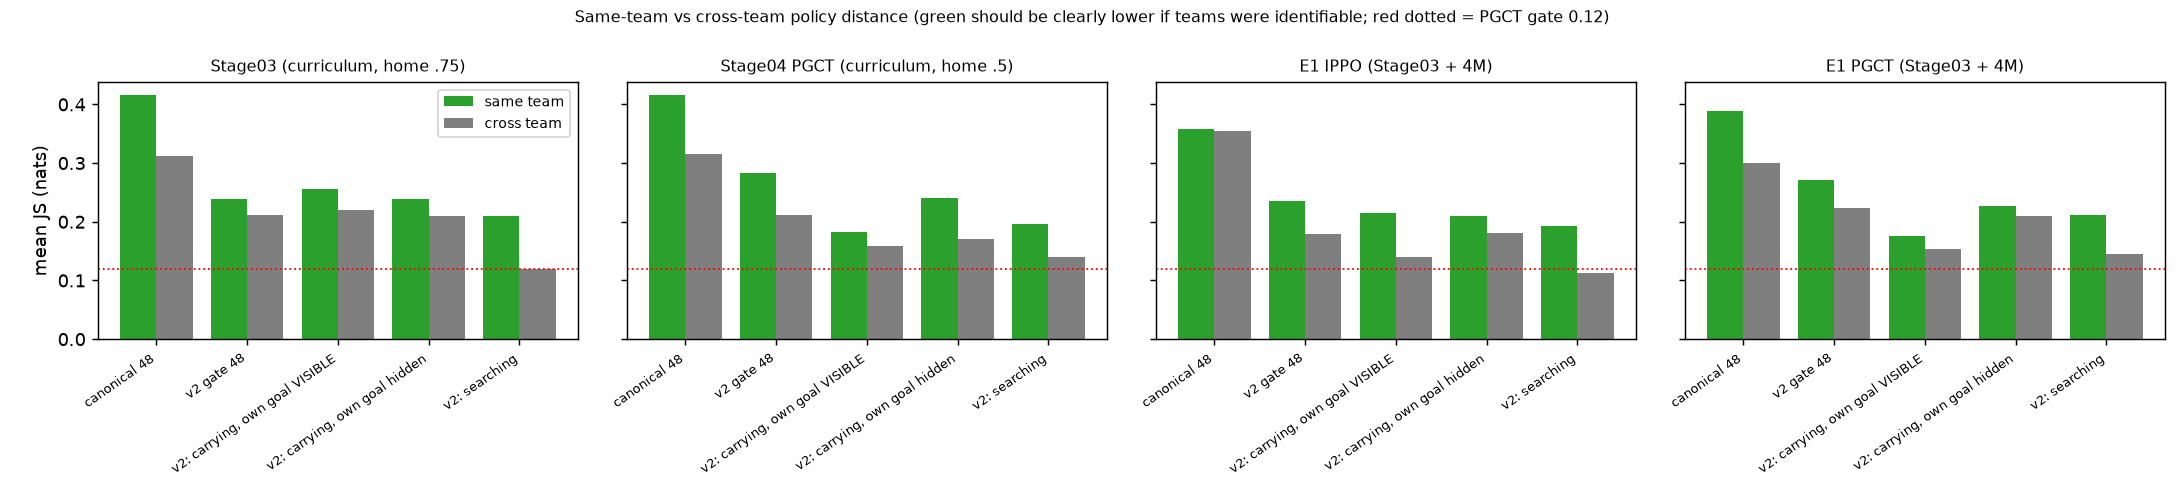
\includegraphics[width=\textwidth]{figures/frozen_probe_same_vs_cross.png}
\caption{고정 E1 모델 4개와 probe 부분집합 5개에서 팀원 사이(초록)와 팀원이 아닌 쌍(회색)의 평균 probe-JS. 부분집합은 canonical
집합, ``적재 중, 목표 안 보임'' 집합, 그리고 transfer 집합의 부분집합(적재 중 자기 목표 보임, 적재 중 목표 안 보임, 탐색)이다.
20개 조합 모두에서 팀원이 덜 비슷하다. 빨간 점선: gate 기준 0.12.}
\end{figure}

\section{커리큘럼 모델의 공간 역할}
\label{app:roles}
\begin{figure}[h]
\centering
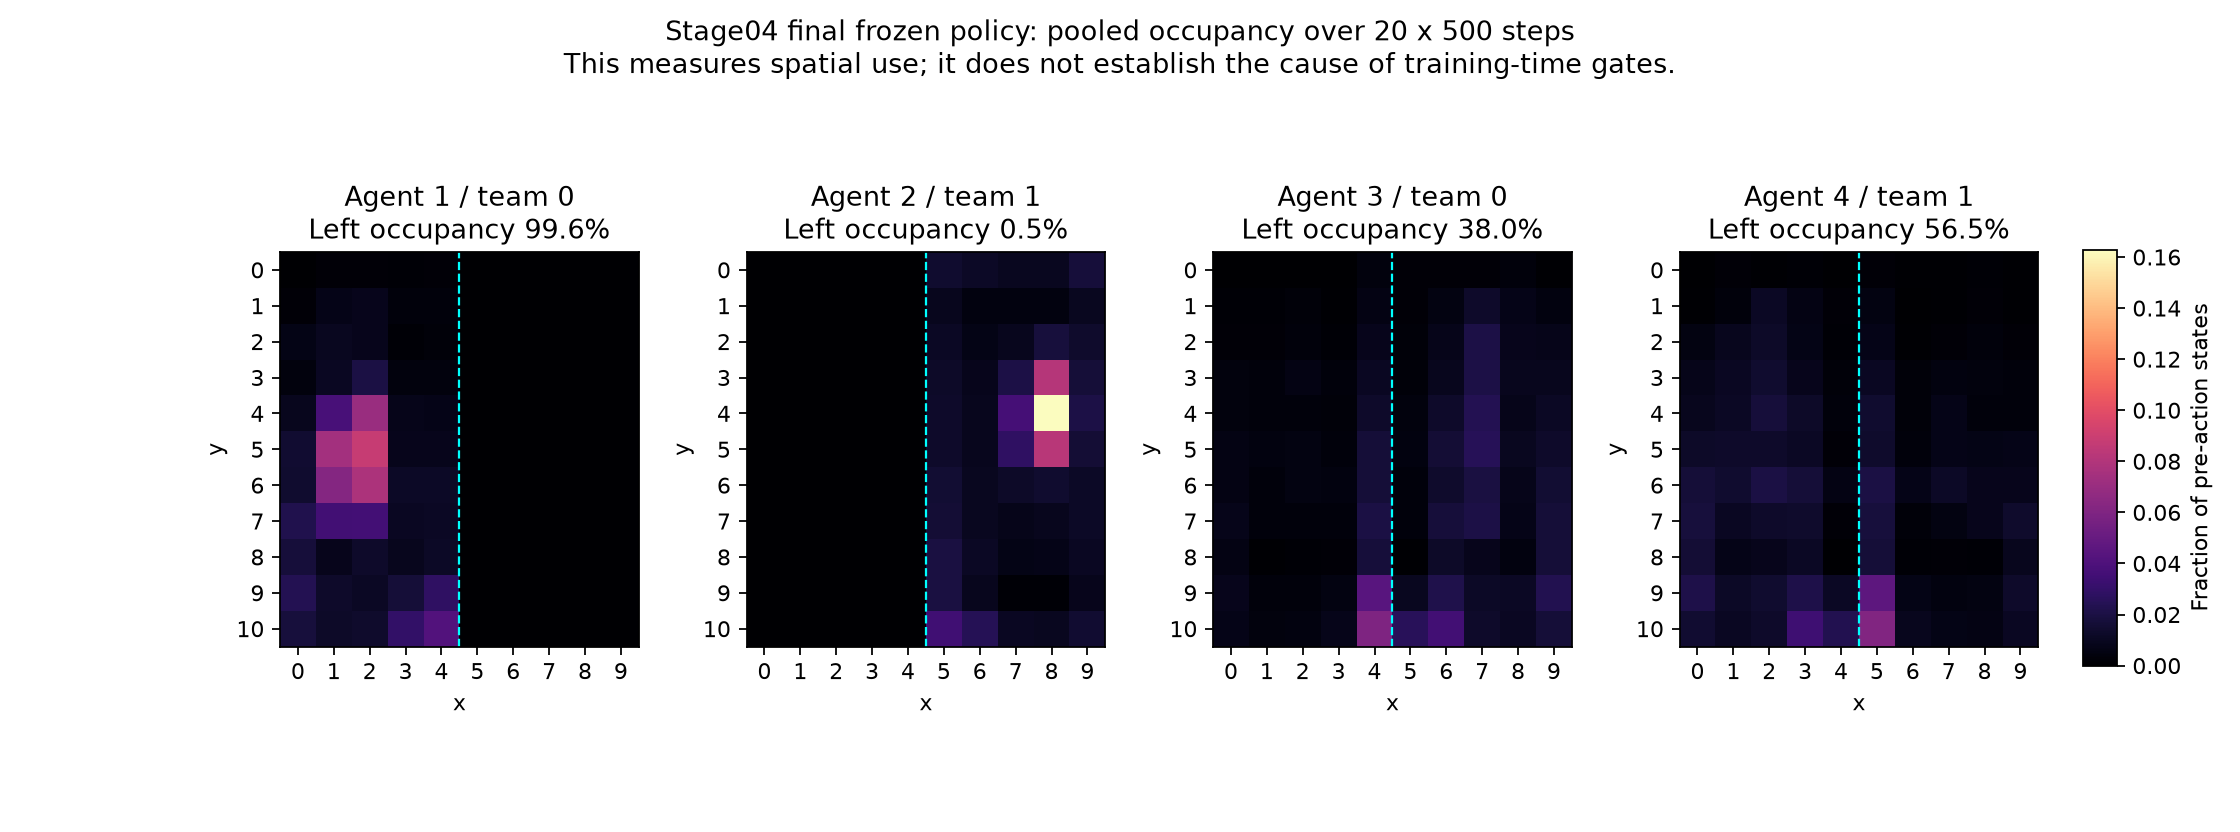
\includegraphics[width=\textwidth]{figures/stage04_occupancy.png}
\caption{고정 커리큘럼 모델(Stage04, 선반의 50\%를 상대 팀 구역에 배치)의 칸 점유, 20$\times$500 step. agent 1과 2는 자기 팀 구역에
머물고, agent 3과 4는 상대 구역에서 선반을 가져온다.}
\end{figure}

\section{선택한 checkpoint의 probe-JS}
\begin{table}[h]
\centering
\small
\begin{tabular}{lcccc}
\toprule
Method & \multicolumn{4}{c}{JS same-team / cross-team at} \\
\cmidrule(lr){2-5}
 & 1M & 2M & 4M & 6M \\
\midrule
IPPO & 0.03 / 0.07 & 0.16 / 0.17 & 0.17 / 0.23 & 0.27 / 0.18 \\
PGCT & 0.07 / 0.06 & 0.16 / 0.16 & 0.17 / 0.15 & 0.26 / 0.19 \\
Oracle-team & 0.07 / 0.06 & 0.16 / 0.18 & 0.31 / 0.19 & 0.29 / 0.23 \\
All-peer & 0.09 / 0.08 & 0.22 / 0.19 & 0.23 / 0.21 & 0.15 / 0.14 \\
\bottomrule
\end{tabular}

\caption{처음부터 학습한 실행에서 팀원 사이 / 팀원이 아닌 쌍 사이의 평균 canonical probe-JS(seed 1개).}
\end{table}

\section{같은 seed에서의 재현성}
\label{app:repro}
\begin{figure}[h]
\centering
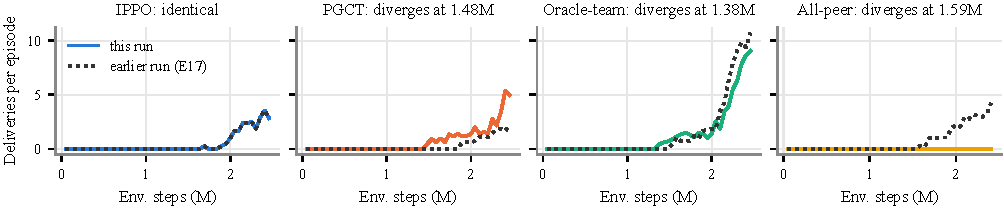
\includegraphics[width=\textwidth]{figures/figA1_reproducibility.pdf}
\caption{같은 seed와 초기 가중치의 두 실행(실선: 이번 실행, 점선: 이전에 중단된 실행). IPPO는 정확히 재현되고, 공유 방식들은
1.4--1.6M step 이후 갈라진다.}
\end{figure}

\section{공통 사전학습 모델에서의 연장 학습}
처음부터 학습하기 전, PGCT와 IPPO를 공통 커리큘럼 checkpoint에서 4M step 더 학습했다(seed 1개). 정규화 배송 AUC는 E1에서
45.86 대 44.57, E2에서 34.17 대 34.24였고, Monte-Carlo return에 대한 최종 critic 정확도는 PGCT가 더 낫지 않았다. 이 단계의 E1에서
gate는 팀원 사이에 한 번도 열리지 않았고(같은 팀 후보 update 4{,}435회 중 0회), 다른 팀 쌍 3--4에는 후보 2{,}525회 중 2{,}005회
열렸다. 이 조건부 결과가 처음부터 학습하는 비교의 동기가 되었다.

\end{document}
